\documentclass{article}

% if you need to pass options to natbib, use, e.g.:
% \PassOptionsToPackage{numbers, compress}{natbib}
% before loading nips_2018

% ready for submission
%\usepackage{nips_2018}

% to compile a preprint version, e.g., for submission to arXiv, add
% add the [preprint] option:
\usepackage[preprint]{nips_2018}

% to compile a camera-ready version, add the [final] option, e.g.:
% \usepackage[final]{nips_2018}

% to avoid loading the natbib package, add option nonatbib:
%\usepackage[nonatbib]{nips_2018}

\usepackage[utf8]{inputenc} % allow utf-8 input
\usepackage[T1]{fontenc}    % use 8-bit T1 fonts
\usepackage{hyperref}       % hyperlinks
\usepackage{url}            % simple URL typesetting
\usepackage{booktabs}       % professional-quality tables
\usepackage{amsfonts}       % blackboard math symbols
\usepackage{nicefrac}       % compact symbols for 1/2, etc.
\usepackage{microtype}      % microtypography
\usepackage[english,ruled,lined]{algorithm2e}
\usepackage{amsmath}
\usepackage{graphicx}
\usepackage{caption}
\usepackage{subcaption}
\bibliographystyle{unsrtnat}

\title{Outcome Prediction for Stock Data}

% The \author macro works with any number of authors. There are two
% commands used to separate the names and addresses of multiple
% authors: \And and \AND.
%
% Using \And between authors leaves it to LaTeX to determine where to
% break the lines. Using \AND forces a line break at that point. So,
% if LaTeX puts 3 of 4 authors names on the first line, and the last
% on the second line, try using \AND instead of \And before the third
% author name.

\author{
  Abel Sapirstein\thanks{Use footnote for providing further
    information about author (webpage, alternative
    address)---\emph{not} for acknowledging funding agencies.} \\
  Department of Computer Science\\
  Harvey Mudd College\\
  Claremont,CA ,91711 \\
  \texttt{asapirstein@hmc.edu} 
}

\begin{document}
% \nipsfinalcopy is no longer used

\maketitle

\begin{abstract}
This work seeks to explore how different cluster algorithms on stock data to automate prediction. K Means and Expectation Maximization are explored and rejected as potential choices. We postulate a hybrid supervised/unsupervised learning schema with a more complex clustering approach that depends on function distance rather than Euclidean distance and instance instance specific clusters.  
\end{abstract}

\section{Introduction}

Outcome prediction and optimization  of partially complete data is a holy grail of sorts. The premise is a simple one, that future behavior of an objective  can be predicted by observing past behavior and current situations. Mathematicians have proposed several solutions to this problem and there currently exist many tools that predict specific types of outcomes quite well. Such tools have broad reaching implications ranging from improving intensive care outcomes(\cite{meiring}) to making lucrative financial choices (\cite{gerlein}). 

Machine Learning is divided into supervised, where labels are supplied, and unsupervised, where labels are not (\cite{murphy}).This paper will focus on using clustering algorithms to automatically label data, which, having been labeled and approved, can then be passed to supervised learning algorithms, such as neural networks. The effectiveness of such clustering schema was assessed on their ability to accurately predict significant behavior in their constituents. Further work in both clustering, and the unsupervised learning models described above, is needed to create an effective approach. 

Stock data provides an easily accessible numeric data with a clear application . Predicting future behavior of stocks has long been the aim of traders, but only recently have accurate algorithmic tools emerged. There are several issues with stock data that can prevent classical regression tools from generating accurate prediction of behaviors. However, a clustering approach that automates labelling is appealing because it would allow for use of more advanced and accurate models of supervised learning. 

There is ample past and current literature on both clustering approaches and advanced supervised learning approaches. We chose to implement two well established clustering algorithms, K Means clustering (\cite{murphy}), and Rubin, Dempster and Laird’s Expectation Maximization algorithm(\cite{dempster}). We hypothesized that the combination of a clustering algorithm to automate trend labeling and a supervised machine learning approach, would be able to predict market behavior at a rate significantly higher than both random chance, classical regression models, and unsupervised learning alone.   


\section{Materials and Methods}
\subsection{Data}
\subsubsection{Training Data}
Training data was composed of the components of the Dow-Jones Industrial Average (DJ-IA) (Appendix A) and was taken from January 1st , 2015  until the end of 2018. There are 30 large cap components to the DJ-IA. This particular index is of interest to us because it is a barometer for the general health of the US economy. Data was taken for each component over a rolling 28 day period. The rationale for this particular choice was that market behavior for a specific day was subject to momentum from the previous four weeks. Furthermore, markets are often subject to large events that affect all components of the DJ-IA . 

The rolling window approach was designed to minimize both the affect of large market events and still provide a large training set. Data was gathered from the Investors Exchange via their API and looked only at the close price for each day. Because of the rolling window size, each data piece could be represented as a point in 28 dimensions. There were approximately 40,000 pieces of data used in the training set. It is worth noting that though the components of the DJ-IA have changed since 2015.For simplicity's' sake, however, the data used queried only current components of the DJ-IA.
\subsubsection{Testing Data}
After models were created, they were validated against the  Standard and Poor 500 index. The S\&P500 is another large cap index. If model created from DJ-IA was representative of generalized large cap behavior, we would expect that the accuracy of the model on the testing data would be approximately equal to that of the training set. The same method was used to generate data but, because the S\&P500 has many more components, we  ended up with approximately 700,000 points. Again, even though the S\&P500 changes quite frequently, we looked only retroactively at the current components. 

\subsection{Clustering Algorithms}
\subsubsection{K Means}
\begin{equation}
    RSS_k = \sum_{\vec{x} \in \vec{\omega_k}}|\vec{x} - \vec{\mu}(\omega_k)|^2 \text {   with   } \vec{\mu}(\omega)= \frac{1}{|\omega|} \sum_{\vec{x}\in \omega}\vec{x}
\end{equation}
K means is one of the most widely used clustering algorithms, with applications ranging from cyber-profiling(Riadi et al., 2016)  to epidemiology (Haughen et al. 2019). It works by creating centroids and grouping points to the centroid that is  the closest Euclidean distance. For this reason the K means algorithm forms circular clusters, and does best at clustering data grouped this way. The objective function (Equation 1) seeks to minimize the total residual sum of squared errors. This is done iteratively via the approach outlined in Algorithm 1. Once the objective function cannot be minimized any further, the algorithm has converged. This algorithm was implemented in Python (3.7) first using the NumPy and SciPy packages. However, for run-time reasons, we switched to the Sci-kit Learn (sklearn)  package’s implementation because our implementation had sub-optimal run-time when compared to sklearn. 
\begin{center}
\begin{algorithm}
 \textit{initialize} $\mu_k$ \;
 \Repeat{\textit{converged} or $(\mu_k)_n = (\mu_k)_{n+1}$}
   {Group each point to nearest cluster center: $z_i = \arg \min_k ||x_0 - \mu_k||^2_2 $\;
   Average all points in grouping and update cluster: $\mu_k = \frac{1}{N_k}\sum_{i:z_i = k} X_i$}
  
  \caption{K Means or Hard EM, from Murphy}
\end{algorithm}
\end{center}
\subsection{Expectation Maximization}
Expectation Maximization (Algorithm 2)  is a markedly more complex clustering algorithm than K means, which is also known as \textbf{Hard EM}, however it hold the promise of being able to recognize non circular trends (\cite{murphy}) . It too has broad applications and has notably used for qualitative genetics(\cite{gosh}[2017]) and to produce readable results in Positive Emission Tomography(\cite{diffey}. We chose to implement  expectation maximization via a Gaussian Mixture Model. We settled on a Gaussian mixture because the noise surrounding our data was approximately normally distributed (see Figure \ref{kmeans:b}). The objective function for EM density distributions seeks to maximize the log-likelihood for a set of parameters. In this case the parameters represent clusters means. Prediction occurs probabilistically by analyzing where a particular point falls in 28 dimensional space and the density distributions dictated by the EM algorithm. Again this algorithm was implemented in Python (3.7) using first NumPy and SciPy, before switching to the Sci-kit Learn implementation for run-time advantages. 
\begin{center}
\begin{algorithm}
 \textit{initialize} $\mu$ as $\frac{\sum_i \vec{r}_i \vec{X}}{r}$ or responsibility of each cluster for each point \;
 \Repeat{\textit{converged} or $(\mu)_n = (\mu)_{n+1}$}
   {\textbf{E Step}: Update responsibilities and calculate expected complete data log likelihood\;
   $\phantom{hashashas} Q(\theta, \theta^{t-1}) = \mathbb{E} \left[ \sum_i \log(p (\x_i,z_i|\theta)\right]$\;
   \textbf{M Step} Optimize $Q$ with respect to $\pi$ and $\theta$\;
    $\phantom{hashashas} \pi = \frac{r}{N}$\;
    Update $\mu$
   }
 \caption{Gaussian Mixture Model from Murphy}
\end{algorithm}
\end{center}
\subsection{Analytic Tools}
We assessed the two models based on how accurately they predicted outcomes. In the training and testing phase correct scores were assigned a value of 1 and incorrect predictions received no value. Furthermore, because from an investing strategy perspective, in our testing phase we also calculated the rate of false negatives, false positives, and true positives and negatives. This was done to more accurately asses the risk that would be shouldered by implementing such a strategy. After all, in the world of investing, false negatives and false positives will loose money. Additionally we tested the robustness of each clustering algorithm by performing linear regression using partially incomplete data.
\begin{figure}[ht]
\centering
\begin{subfigure}{.5\textwidth}
  \centering
  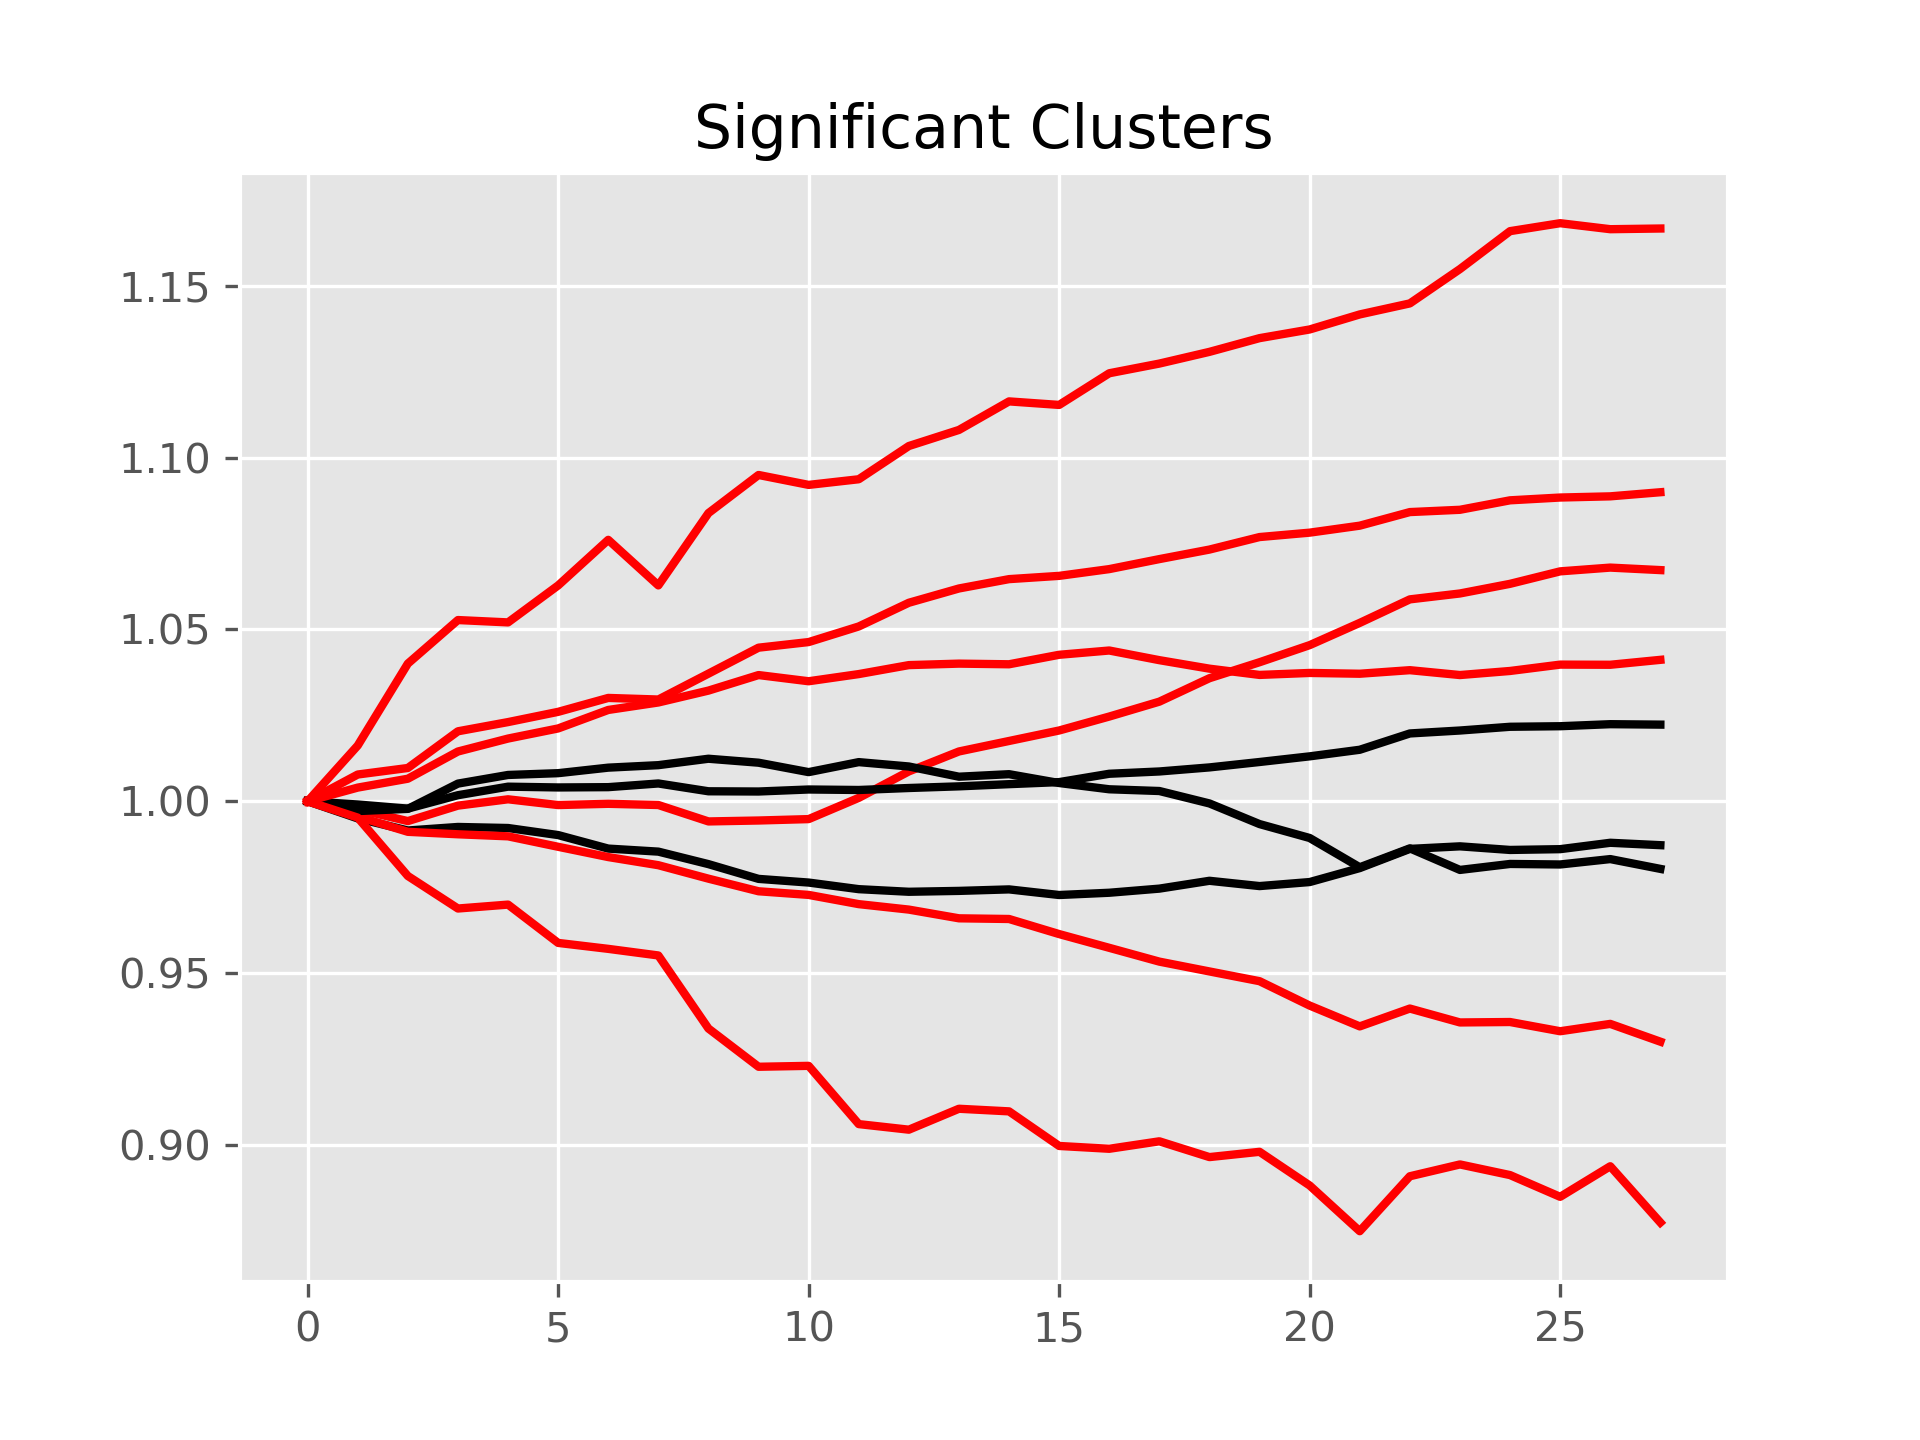
\includegraphics[width=\linewidth]{SigClus.png}
  \caption{Time series of centroid clusters: red indicates significance}
  \label{kmeans:a}
\end{subfigure}%
\begin{subfigure}{.5\textwidth}
  \centering
  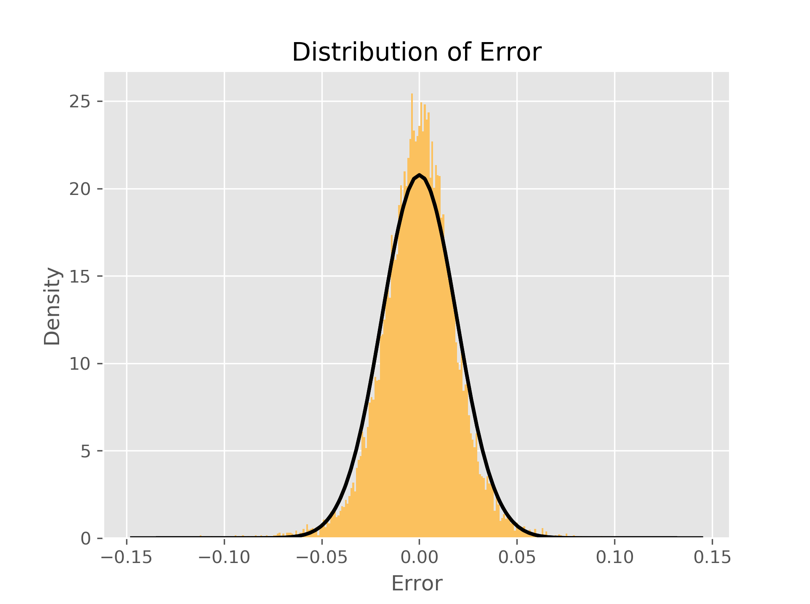
\includegraphics[width=\linewidth]{hist.png}
  \caption{Histogram showing distribution of errors}
  \label{kmeans:b}
\end{subfigure}
\caption{Results from K Means Clustering}
\label{kmeans}
\end{figure}
\section{Results}

K means was run with 9 clusters. This number is relatively small because we did not want to potentially over-fit the data and wanted to highlight ubiquitous trends. In both the testing and the validation set, we found 6 of the 9 clusters generated distributions had distributions that we could state with 95\% confidence were not equivalent to 1, indicating potential for a predictable yield. However these 6 clusters did not encompass a significant majority of the data, only 50\% of inputs fell into these clusters. Significant clusters are shown in red and insignificant ones are shown in black (Figure \ref{kmeans:a}) . When this model was validated, it performed slightly better, with 53\% data from the validation set falling into the significant categories. Additionally the error was relatively normally distributed with a standard deviation of 1.9\% percent from cluster mean. 
\begin{figure}[h]
\begin{subfigure}{.35\textwidth}
  \centering
  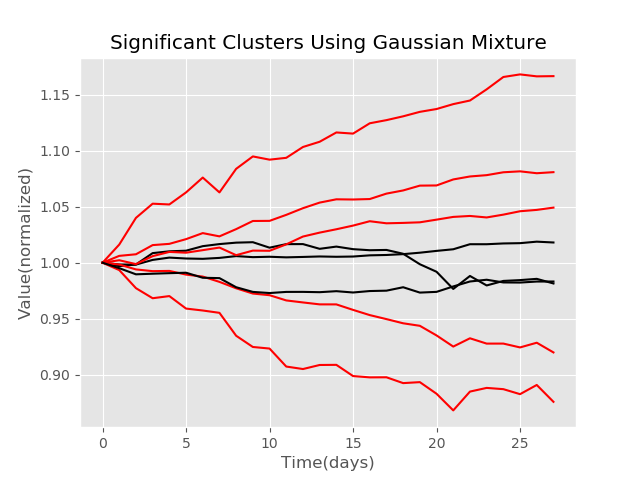
\includegraphics[width=\linewidth]{sigfig.png}
  \caption{Time series of mean cluster: red indicates significance}
  \label{gmm:a}
\end{subfigure}%
\begin{subfigure}{.65\textwidth}
  \centering
  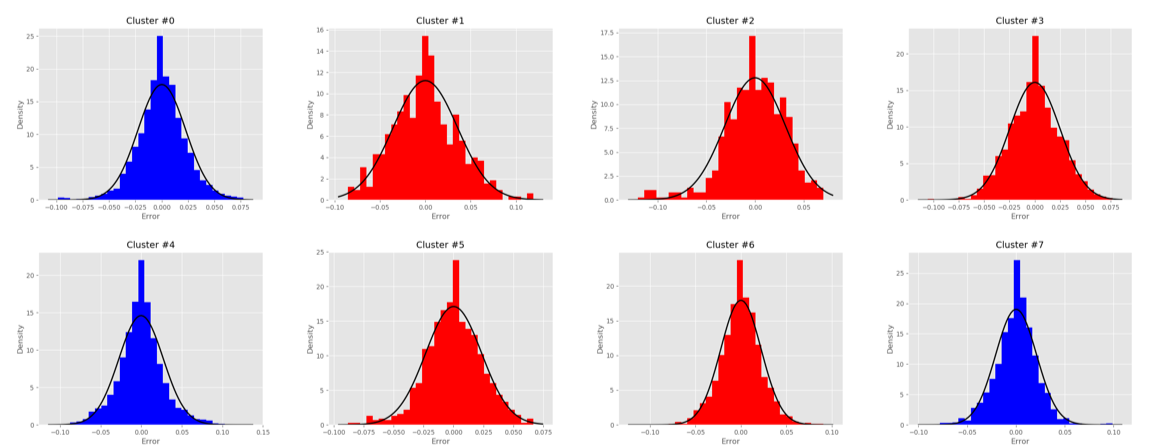
\includegraphics[width=\linewidth]{hists.png}
  \caption{Histogram showing distribution of errors among clusters}
  \label{gmm:b}
\end{subfigure}
\caption{Results from GMM Probability Density}
\label{gmm}
\end{figure}

	The Gaussian mixture model was trained with 8 clusters, again to elucidate significant trends in generalized data. In both the testing and validation sets, 5 of the 8 clusters were distributed in a way that was significantly (95\% confidence) different from one, indicating potential for a predictable yield. There was significantly fewer points encompassed in the significant clusters, when compared to K means. In the training data, only 34\% of inputs were classified (with 95\% confidence) in significant clusters. The deviation within the cluster from the centroid ( Euclidean) is showing in Figure 4b and all are normally distributed.  In the testing data, the model again performed slightly better, 38\% of data was predicted to fall in significant categories. 
\section{Discussion}
\subsection{Kmeans}
Neither clustering model performed as desired. Kmeans clustering performed either at or slightly above random chance. However, because all of its predicting power was in high movement clusters (Figure \ref{kmeans:a}), this is not particularly useful. Furthermore because a linear regression scales linearly, we need to include upwards of 80\% of a cluster to accurately predict outcome ( Figure \ref{fig:accur}). As expected, this classical method of outcome prediction is not particularly accurate. This is due to the assumption of Euclidean distance that does not accurately represent the complex array of factors that impact stock prices.
\begin{figure}[h]
    \centering
    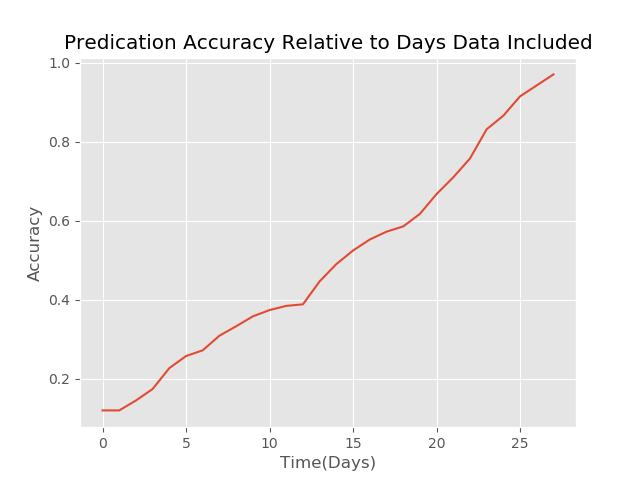
\includegraphics[width = .5\linewidth]{Accuracy.png}
    \caption{Accuracy Relative to Days Included}
    \label{fig:accur}
\end{figure}
\subsection{GMM}
	Surprisingly the GMM performed even worse than K-means clustering. We could only confidently predict outcomes with a maximal accuracy of 38\%. In an economic sense, this makes sense, most stocks do not move a significant amount and are closely clustered around 1 , when we normalize their values to a starting value. Edge cases are points that have significant movement above or below 1 but are not clustered as such. K means is remarkably better at categorizing such points because it relies on a hard threshold rather than the continuous probability distribution of the GMM which seems to obfuscate part of the data. We did not yet develop a solid metric for incomplete data prediction, because partial data is dependent on the probability distributions of each cluster. 

\section{Conclusion}
\subsection{Unsupervised Learning}
	We did not continue with the originally outlined approach because of the lackluster performance of these clustering approaches. The central flaw of this approach is the used of Euclidean distance. As mentioned above future stock behavior can be affected by more than just the previous price. If a market is suddenly saturated by demand, and volume remains low, the price is likely to increase at a much higher rate that if the same demand hits a high volume market. Furthermore, not all time series represent the same events. If the 28 day window includes a end of quarter report, we would expect that the stocks price would be dictated much more heavily by if earnings met expectations than past behavior. Past behavior can partially be an indicator of how likely earnings are to meet expectations, or at least market perception of this. 
\subsection{Next Steps}
\begin{figure}[h]
    \centering
    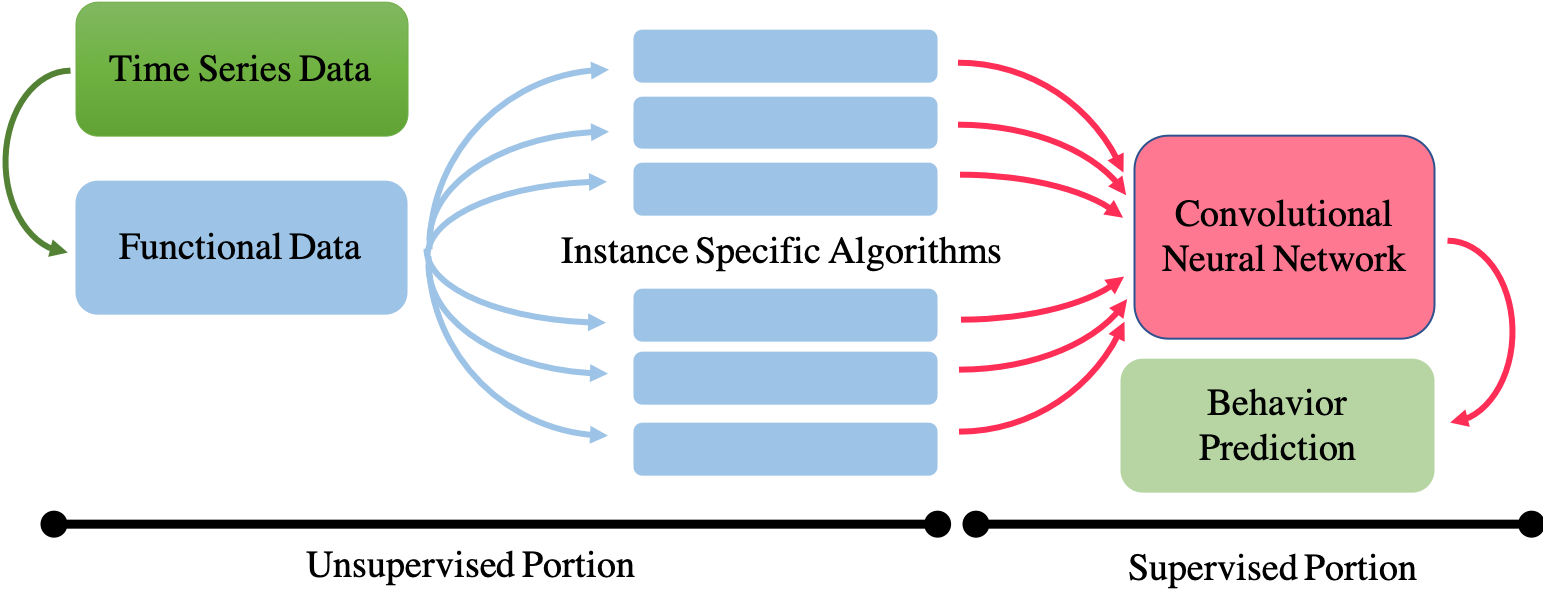
\includegraphics[width =\linewidth]{workflow.png}
    \caption{Proposed Mixing of Supervised and Unsupervised Learning}
    \label{fig:mix}
\end{figure}
A relatively simple model that includes only  a Euclidean distance metric does not accurately account for these complex phenomena.  Thus before our model can begin the supervised learning phase, we must first adjust the distance approach that we are using. Functional analysis may provide a better distance metric if instead of representing the data as a particular point in 28 dimensions, we represented the same time series as a function, we might be able to better cluster the data. 

Furthermore if we know that a particular model is well suited for a particular scenario, the global model should run. For example, we can train a functional model only upon end of quarter data. Thus when it comes time to attempt to predict the behavior following a quarterly earnings report, we ought to focus our global model on this functional model. This approach, where we isolate anomalous models, and train functional sub models on them would likely yield better results. 
	
The aim of this project still stands, to create a hybrid approach to stock performance models. However our current approach fails to accurately label stocks, and a model that accurately categorizes stocks is needed before we can move towards implementation of a supervised learning model. The final model will be tuned to more accurately predict outcome values. It will do this by first modifying the clustering approach to incorporate  both more representative data (converting to functional data rather than Euclidean spaces) and using instance specific algorithms to catch special cases that should be compared within similar instances. Only after this approach is successfully implemented will the labeling schema be passed to a convolutional neural network. This will create several hidden layers and hopefully lead to more accurate prediction. 



\section*{References}

References follow the acknowledgments. Use unnumbered first-level
heading for the references. Any choice of citation style is acceptable
as long as you are consistent. It is permissible to reduce the font
size to \verb+small+ (9 point) when listing the references. {\bf
  Remember that you can use more than eight pages as long as the
  additional pages contain \emph{only} cited references.}
\medskip
\bibliography{midterm}
\newpage
\section*{Appendix A: Dow Jones Industrial Average}
\begin{center}
\begin{table}[h]
\begin{tabular}{lll}
Dow Jones Industrial Average                &               &              \\
Company Name                                & Ticker Symbol & Weighting \% \\
3M Company                                  & MMM           & 5.39\%       \\
American Express Company                    & AXP           & 2.80\%       \\
Apple Inc.                                  & AAPL          & 5.91\%       \\
Caterpillar Inc.                            & CAT           & 3.45\%       \\
Chevron Corporation                         & CVX           & 3.14\%       \\
Cisco Systems, Inc.                         & CSCO          & 1.23\%       \\
DowDuPont Inc.                              & DWDP          & 1.50\%       \\
Exxon Mobil Corporation                     & XOM           & 2.17\%       \\
Intel Corporation                           & INTC          & 1.21\%       \\
International Business Machines Corporation & IBM           & 3.48\%       \\
Johnson \& Johnson                          & JNJ           & 3.71\%       \\
JPMorgan Chase \& Co.                       & JPM           & 2.85\%       \\
McDonald's Corporation                      & MCD           & 4.46\%       \\
Merck \& Co., Inc.                          & MRK           & 1.94\%       \\
Microsoft Corporation                       & MSFT          & 2.94\%       \\
NIKE, Inc.                                  & NKE           & 2.01\%       \\
Pfizer Inc.                                 & PFE           & 1.19\%       \\
The Boeing Company                          & BA            & 9.53\%       \\
The Coca-Cola Company                       & KO            & 1.23\%       \\
The Goldman Sachs Group, Inc.               & GS            & 5.94\%       \\
The Home Depot, Inc.                        & HD            & 4.79\%       \\
The Procter \& Gamble Company               & PG            & 2.32\%       \\
The Travelers Companies, Inc.               & TRV           & 3.32\%       \\
The Walt Disney Company                     & DIS           & 3.16\%       \\
United Technologies Corporation             & UTX           & 3.39\%       \\
UnitedHealth Group Incorporated             & UNH           & 7.02\%       \\
Verizon Communications Inc.                 & VZ            & 1.47\%       \\
Visa Inc.                                   & V             & 3.77\%       \\
Walgreens Boots Alliance, Inc.              & WBA           & 2.08\%       \\
Walmart Inc.                                & WMT           & 2.60\%      
\end{tabular}
\end{table}
\end{center}
\end{document}
